\documentclass{article}
\usepackage[utf8]{inputenc}
\usepackage{graphicx}


\title{Lab 03- ARP Poisoning and DHCP Security}
\author{Matthew Belanger}
\date{\today}

\begin{document}

\maketitle

\newpage

% SECTION 1

% TASK 1

\section{Task 1: ARP Poisoning Attack}

\subsection{Network configurations and ARP tables before and after the attack.}

\subsection{Scapy scripts used.}

\subsection{Screenshots demonstrating the success of the attack, including Wireshark captures.}

\subsection{Discussion on mitigation strategies.}

\newpage

% TASK 2

\section{Task 2: Security Analysis of The DHCP}

\subsection{Start Wireshark open the enclosed pcap trace file and list all the DHCP packets in the trace. Use
screenshots to support your answer.}

See Figure \ref{fig:pcap_dhcp}

\begin{figure}[h]
    \centering
    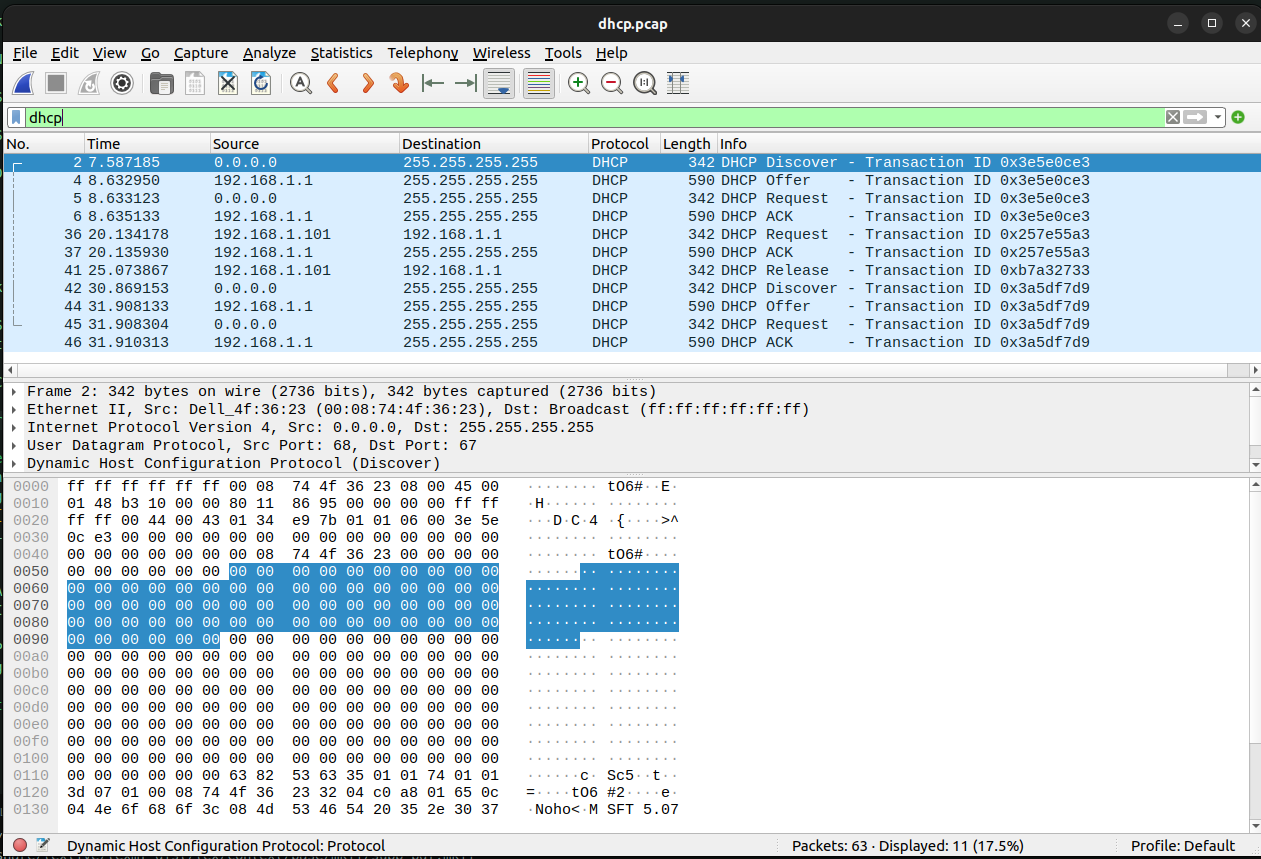
\includegraphics[width=0.8\textwidth]{task2/dhcp_wireshark.png}
    \caption{DHCP Packet List}
    \label{fig:pcap_dhcp}
\end{figure}

\subsection{Create a Finite State Machine model for the DHCP process.}
 
See Figure \ref{fig:dhcp_fsm}

\begin{figure}[h]
    \centering
    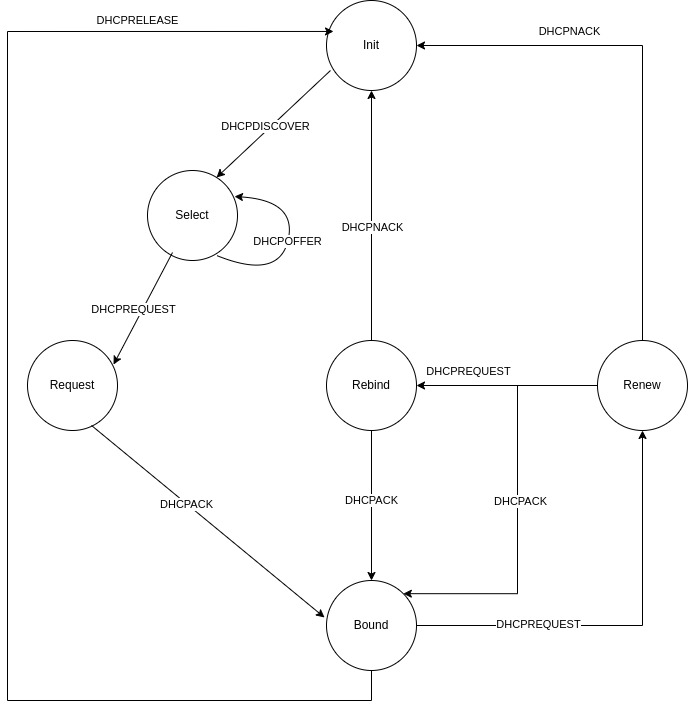
\includegraphics[width=0.8\textwidth]{task2/DHCP_FSM.jpg}
    \caption{DHCP Finite State Machine}
    \label{fig:dhcp_fsm}
\end{figure}

\subsection{Apply the STRIDE methodology to the FSM model of DHCP to identify potential security threats.
For each STRIDE element, identify possible vulnerabilities in the DHCP process.}

\subsubsection{Spoofing}

\subsubsection{Tampering}

\subsubsection{Repudiation}

\subsubsection{Information Disclosure}

\subsubsection{Denial of Service}

\subsubsection{Elevation of Privilege}

\subsection{Propose mitigation strategies for each identified vulnerability. This could involve protocol enhance-
ments, configuration changes, or additional security mechanisms.}

\subsubsection{Spoofing}

\subsubsection{Tampering}

\subsubsection{Repudiation}

\subsubsection{Information Disclosure}

\subsubsection{Denial of Service}

\subsubsection{Elevation of Privilege}

\end{document}
